\documentclass[conference]{IEEEtran}
\IEEEoverridecommandlockouts
% The preceding line is only needed to identify funding in the first footnote. If that is unneeded, please comment it out.
\usepackage{cite}
\usepackage{amsmath,amssymb,amsfonts}
\usepackage{algorithmic}
\usepackage{graphicx}
\usepackage{textcomp}
\usepackage{xcolor}
\def\BibTeX{{\rm B\kern-.05em{\sc i\kern-.025em b}\kern-.08em
    T\kern-.1667em\lower.7ex\hbox{E}\kern-.125emX}}

\makeatletter
\newcommand{\linebreakand}{%
  \end{@IEEEauthorhalign}
  \hfill\mbox{}\par
  \mbox{}\hfill\begin{@IEEEauthorhalign}
}
\makeatother
\begin{document}

\title{A Framework for Understanding \\ Research Software Sustainability}

\author{\IEEEauthorblockN{Neil P. Chue Hong}
\IEEEauthorblockA{\textit{Software Sustainability Institute \& EPCC} \\
\textit{University of Edinburgh}\\
Edinburgh, United Kingdom \\
https://orcid.org/0000-0002-8876-7606} \\
\and
\IEEEauthorblockN{Matthew Bluteau}
\IEEEauthorblockA{\textit{Culham Centre for Fusion Energy} \\
\textit{UK Atomic Energy Authority}\\
Culham, United Kingdom \\
https://orcid.org/0000-0001-9498-8475}
\linebreakand
\IEEEauthorblockN{Anna-Lena Lamprecht}
\IEEEauthorblockA{\textit{Department of Information and Computing Sciences} \\
\textit{Utrecht University}\\
Utrecht, The Netherlands \\
https://orcid.org/0000-0003-1953-5606}
\and
\IEEEauthorblockN{Zedong Peng}
\IEEEauthorblockA{\textit{Department of Electrical Engineering and Computer Science} \\
\textit{University of Cincinnati}\\
Cincinnati, United States of America\\
https://orcid.org/0000-0002-5071-1586}
}

\maketitle

\begin{abstract}
Software sustainability relies on many different aspects: code quality and design, maintenance, governance, infrastructure, community engagement, and of course funding. Understanding what the requirements are for sustaining research software is often hampered because one size doesn’t fit all. This position paper proposes a framework for categorising the different types of research software, suggests how this framework can be used to identify good practice for each aspect, and proposes areas for future research.
\end{abstract}

\begin{IEEEkeywords}
software sustainability, research software, maturity model, testing
\end{IEEEkeywords}

\section{Why a framework is useful}
When evaluating potential practices to support software sustainability, it can be difficult to identify what approaches work best. Should you use continuous integration for simple scripts? What level of documentation is appropriate for the notebook used to analyse your data? When should you hire a community manager?

This is principally because each choice you make must be balanced against the effort to implement, and the number of times you will benefit from doing it. A framework allows software owners to evaluate the practices they should be considering based on an assessment of “where” their software is at present. It also makes it easier to interpret the types of guidance available, much in the same way that frameworks used in education and training help learners understand whether a course is at an appropriate level for them.

Many existing frameworks have been proposed for software. From the first cost model for software reuse developed at CMU's Software Engineering Institute \cite{Holibaugh}, there have been several models proposed for software reuse including the Reuse Maturity Model \cite{Koltun}, the reuse model for DARPAs STARS program \cite{Frazier}, the CMMI \cite{CMMI}, and the Software Sustainability Maturity Model \cite{Gardler}, and - potentially the most widely used - Technology Readiness Levels. However most of these frameworks assess the software from the perspective of the user, not the developer/owner. Typically, they define levels based on the availability and readiness for use by someone else.

More recently, other approaches have looked at defining levels based on maturity and how widely software has been shared or published. These include application classes for software produced by the German Aerospace Center \cite{Schlauch} and the schematic stages of open community for research software proposed at an URSSI workshop \cite{Benthall}. Chue Hong \cite{Chue Hong} also looked at comparisons with levels of startups, as defined by the Startup Genome Project (colloquially known as Marmer stages) \cite{Marmer}, and other research has looked at the role of types of project teams \cite{Cohoon}.


\section{Defining a framework}

Building on the work of the various frameworks, we define a set of Research Software Levels (Table \ref{ResearchSoftwareLevels}) which are characterised using a number of dimensions that are important for assessing the ``level'' of a piece of research software. Users refers to the scope of those using the software. Distribution refers to how widely the software itself is shared, both in terms of the numbers of people who can use it and the closeness of their relationship to the developer. Reuse refers to how often the software is expected to be reused after that point. Support refers to the expectation of what happens when the software does not work as expected.

{\renewcommand{\arraystretch}{2}
\begin{table*}[htbp]
\caption{Research Software Levels}
\begin{center}
\begin{tabular}{|p{0.1\linewidth}|p{0.15\linewidth}|p{0.2\linewidth}|p{0.2\linewidth}|p{0.2\linewidth}|}
\hline
\textbf{Level} & \textbf{Expected users} & \textbf{Expected distribution} & \textbf{Expected reuse} & \textbf{Expected support} \\
\hline
\textbf{0 - Personal} &
Developer only &
Private to developer (typically unlicensed) &
Only while required &
None \\
\hline
\textbf{1 - Research} &
Internal to team & 
Often only published to accompany an associated publication &
As long as research is being conducted / reproduced &
Limited to fixing issues preventing research \\
\hline
\textbf{2 - Supported} &
Others in community, mostly collaborators &
Often published on a website or in a public code repository. License. &
As long as research is being conducted / reproduced &
Best effort unless funded \\
\hline
\textbf{3 - Product} &
Wide range of users  &
Releases formally and widely distributed with clear license. &
Until release is withdrawn or superceded &
Defined levels of support, roadmap \\
\hline
\textbf{4 - Critical} &
Used in critical applications &
Releases formally and widely distributed with clear license. &
Until any legal requirement is discharged &
Frequent level of maintenance \\
\hline
\end{tabular}
\label{ResearchSoftwareLevels}
\end{center}
\end{table*}
}

As examples of the different levels, we might have:
\begin{itemize}
    \item Level 0 - Personal: a short convenience script used once to process a dataset, a notebook used to explore an initial concept
    \item Level 1 - Research: software written to generate results in a paper
    \item Level 2 - Supported: a software model used by collaborators at different institutions
    \item Level 3 - Product: a widely used software library, a commercial application
    \item Level 4 - Critical: a widely used key package, a mission critical piece of software associated with a large experiment
\end{itemize}

These are similar to the application classes defined in \cite{Schlauch}, but we further segment their application class 1 into Levels 1 and 2 to distinguish between software primarily used in a small team who are all contributing and software where some users are collaborators but not contributors. We also define expected dimensions to help categorise software into the different levels.


\section{Applying the framework}
With the definition of these different levels, we can use this to understand which practices, approaches, tools or infrastructure are best suited to a particular level. For instance, in Figure \ref{infrastructure}, we can identify infrastructure for collaboration and communication, using a similar approach to that in the book Producing Open Source Software \cite{Fogel}. Level 4 - Critical is omitted in this figure, but might include Customer Support infrastructure.

\begin{figure*}[htbp]
\centerline{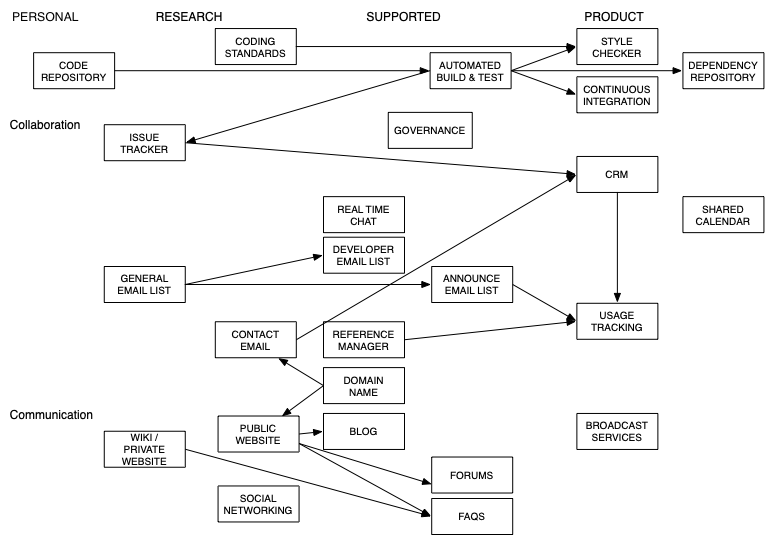
\includegraphics[width=\textwidth]{infrastructure.png}}
\caption{Collaboration and communication infrastructure appropriate at different research software levels.}
\label{infrastructure}
\end{figure*}

We can also look at approaches to quality assurance, encompassing both software and scientific testing. 

{\renewcommand{\arraystretch}{2}
\begin{table*}[htbp]
\caption{Research Software Levels}
\begin{center}
\begin{tabular}{|p{0.1\linewidth}||p{0.2\linewidth}|p{0.3\linewidth}|p{0.3\linewidth}|}
\hline
\textbf{Level} & 
\textbf{Validation requirements} & 
\textbf{Testing requirements} & 
\textbf{Testing approaches} \\
\hline
0 - Personal &
Reassure researcher that data isn’t incorrect &
Test that plausible results appear to be generated, i.e intuition &
Manual/interactive checking against test data  \\
\hline
\multicolumn{3}{|l|}{Level 0 → 1} &
Turn manual tests into software tests \\
\hline

1 - Research &
Reasonable reproducibility of published result &
Tests cover core aspects of the science &
Small number of system tests / unit tests  \\
\hline
\multicolumn{3}{|l|}{Level 1 → 2} &
Automate testing  \\
\hline
2 - Supported &
Algorithms and models are accurately implemented &
Checking against data formats, testing performance &
Use of test frameworks  \\
\hline
\multicolumn{3}{|l|}{Level 2 → 3} &
Apply regression testing on key functionality  \\
\hline
3 - Product &
Performs as expected in range of conditions &
Stress testing, testing usability and robustness, including detection of concurrency and memory errors  &
Property based testing. Acceptance testing. Performance analysis. Fault localization \\
\hline
\multicolumn{3}{|l|}{Level 3 → 4} &
Independent assessment  \\
\hline
4 - Critical &
Legal or reputational protection &
Full coverage and traceability &
Testing compliance to standards. Security analysis \\
\hline
\end{tabular}
\label{testing}
\end{center}
\end{table*}
}

Here we note that we the general approach for research software is perhaps different from the IT industry (e.g. as described in Figure 1 of \cite{Zamansky}), where unit tests are likely to be implemented before system tests. We hypothesise that this is because it is easier for researchers to implement end-to-end regression tests (i.e. system tests) than unit tests. For example, they get a number that they are confident is right from their code, and they implement that as a test for the "gold" result, or they automate a system test that uses a known set of input and output files. This table could be extended to identify different static analysis approaches that can be useful applied at each level, including linting and formal verification.

Similarly, we could use this approach to understand the appropriate requirements and approaches to funding, community engagement and governance / leadership that improve software sustainability. 

An important thing to note is that software can move between levels, e.g. because it is seen as useful by a wider set of users, and all software doesn’t start at Level 0. It is important to identify the approaches that allow a software project to meet the more stringent requirements if it moves up a level.


\section{Further research}

There are a number of avenues of research that can be undertaken to improve on this framework: 
\begin{itemize}
    \item Similar approaches to the Startup Genome Report \cite{Marmer} and in Cohoon and Howison's work \cite{Cohoon} could be used to examine a large cohort of research software projects to give confidence that the levels are sensible and distinct.
    \item Surveys can be run, based on this framework, to identify the common practices in use at each level in different communities.
    \item Comparison against approaches taken in industry to use similar frameworks to identify best practice at different stages of maturity
\end{itemize}

\section{Conclusions}

We present a framework for categorising research software into different levels based on four key dimensions and utilise this framework to suggest how to identify the appropriate infrastructure and testing approaches required for each level. Further research is required to better understand whether the examples we provide represent the current status of research software infrastructure and testing, but we believe that the framework provides a structured way to represent the different requirements for software sustainability for different software.

\newpage

\section*{Acknowledgements}

NCH is supported by EPSRC, BBSRC, ESRC, NERC, AHRC, STFC and MRC grant EP/S021779/1 for the UK Software Sustainability Institute.

The original ideas for Table \ref{ResearchSoftwareLevels} and Figure \ref{infrastructure} were developed by NCH. Table \ref{testing} is adapted from an idea by A-LL, MB, NCH and ZP developed at SE4Science’21. Tracy Teal provided feedback on some of the ideas in this document.


\begin{thebibliography}{00}

\bibitem{Benthall} Benthall, S.P. (2019). Software Incubator Workshop: A Synthesis. Accessed on 16th June 2021 from: http://urssi.us/blog/2019/02/25/software-incubator-workshop-a-synthesis/

\bibitem{Chue Hong} Chue Hong, N. P. (2015). Why developing research software is like a startup (and why this matters). International Symposium on Grids and Clouds 2015 (ISGC2015). Available from: https://www.slideshare.net/npch/why-developing-research-software-is-like-a-startup-and-why-this-matters

\bibitem{CMMI} CMMI Product Team, 2006. CMMI for Development, Version 1.2. SEI Identifier: CMU/SEI-2006-TR-008.

\bibitem{Cohoon} Cohoon, J. and Howison, J. (2018). Routes to Sustainable Software: Transitioning to Peer Production. Proceedings of the 2018 Annual Meeting of the Academy of Management. DOI: https://doi.org/10.5465/AMBPP.2018.12182abstract
 
\bibitem{Fogel} Fogel, K. (2020). Producing Open Source Software (2nd Edition). O’Reilly. Available from https://producingoss.com/

\bibitem{Frazier} Frazier, T.P., and Bailey, J.W. 1996. The Costs and Benefits of Domain-Oriented Software Reuse: Evidence from the STARS Demonstration Projects. Accessed on 16th June 2021
from: https://apps.dtic.mil/sti/citations/ADA312063

\bibitem{Gardler} Gardler, R. 2013. Software Sustainability Maturity Model. Accessed on 16th June 2021 from: http://osswatch.ac.uk/resources/ssmm

\bibitem{Holibaugh} Holibaugh, R et al. 1989. Reuse: where to begin and why. Proceedings of the conference on Tri-Ada '89: Ada technology in context: application, development, and deployment. p266-277. DOI: 10.1145/74261.74280.

\bibitem{Koltun} Koltun, P. and Hudson, A., (1991). A reuse maturity model. 4th Annual Workshop on Software Reuse, Hemdon, Virginia: Center for Innovative Technology

\bibitem{Marmer} Marmer, M., Herrmann, B.L., Dogrultan, E., Berman, R. (2011). Startup Genome Report: A new framework for understanding why startups succeed. Version 1.0. Startup Compass.  

\bibitem{Schlauch} Schlauch, T., Meinel, T., Haupt, C. (2018). DLR Software Engineering Guidelines, Version 1.0.0, Zenodo. DOI: https://doi.org/10.5281/zenodo.1344612

\bibitem{Zamansky} Zamansky, A., Spichkova, M., Rodriguez-Navas, G., Herrmann, P., and Blech, J. O. (2018). Towards Classification of Lightweight Formal Methods. Proceedings of the 13th International Conference on Evaluation of Novel Approaches to Software Engineering. https://doi.org/10.5220/0006770803050313


\end{thebibliography}
\vspace{12pt}

\end{document}
